\documentclass[12pt, letterpaper]{report}
%\usepackage[paperwidth=8.5in, paperheight=11in]{geometry}
%\special{papersize=8.5in,11in}
%\usepackage[letterpaper]{geometry}
%\usepackage[pass,letterpaper]{geometry}
%\usepackage{geometry}
\usepackage[english]{babel}
\usepackage{natbib}
\usepackage{url}
\usepackage[utf8x]{inputenc}
\usepackage{amsmath}
\usepackage{graphicx}
\graphicspath{{images/}}
\usepackage{parskip}
\usepackage{fancyhdr}
\usepackage{vmargin}
\usepackage{lipsum}
%Saeed packages
%\usepackage[caption=false]{subfig}
\usepackage{amsmath,graphicx,url,bbm}
\usepackage{amssymb}
\usepackage{tabularx,esdiff,algorithm, mathtools,xparse,subcaption,subfiles}
\usepackage{algorithmicx}
\usepackage{algpseudocode}
\renewcommand{\algorithmicrequire}{\textbf{Input:}}
\renewcommand{\algorithmicensure}{\textbf{Output:}}
\DeclarePairedDelimiter{\norm}{\lVert}{\rVert}
\usepackage{color}
\usepackage{booktabs}
\usepackage{multirow}
%End of Saeed packages
\usepackage[dvipsnames]{xcolor}

%Bob packages not already included above
\usepackage{titlesec} % For \subsubsubsection
%\usepackage{hyperref} % For \subsubsubsection and \texorpdfstring.
\usepackage[hidelinks]{hyperref} % For \subsubsubsection and \texorpdfstring

\usepackage{booktabs}
\usepackage{multirow}
%\usepackage{siunitx}
\usepackage{makecell}
%\usepackage{dashrule}
\usepackage{xcolor}
\usepackage{colortbl}

%End of Bob packages

%%%%%%%%%%%%%%
% New command to draw "DRAFT" watermark on every page.
\newcommand{\drawwatermark}
{
%\usepackage{draftwatermark}
\usepackage[printwatermark]{xwatermark}
%\newwatermark*[allpages,color=red!15,angle=45,scale=2.7,xpos=0,ypos=0]{\bfseries\sffamily %DRAFT}
\usepackage{tikz}
\newsavebox\mybox
\savebox\mybox{\tikz[color=red,opacity=0.1]\node{DRAFT};}
\newwatermark*[
  allpages,
  angle=45,
  scale=7,
  xpos=0,
  ypos=5
]{\usebox\mybox}
}

% Comment or uncomment the following line to put a "DRAFT" watermark on every page
%\drawwatermark

%%%%%%%%%%%%%%

%%%%%%%%%%%%%%
%
% Define \subsubsubsection
%
\usepackage{titlesec}
%\usepackage{hyperref}   %This is already included above

\titleclass{\subsubsubsection}{straight}[\subsection]

\newcounter{subsubsubsection}[subsubsection]
\renewcommand\thesubsubsubsection{\thesubsubsection.\arabic{subsubsubsection}}
\renewcommand\theparagraph{\thesubsubsubsection.\arabic{paragraph}} % optional; useful if paragraphs are to be numbered

\titleformat{\subsubsubsection}
  {\normalfont\normalsize\bfseries}{\thesubsubsubsection}{1em}{}
\titlespacing*{\subsubsubsection}
{0pt}{3.25ex plus 1ex minus .2ex}{1.5ex plus .2ex}

\makeatletter
\renewcommand\paragraph{\@startsection{paragraph}{5}{\z@}%
  {3.25ex \@plus1ex \@minus.2ex}%
  {-1em}%
  {\normalfont\normalsize\bfseries}}
\renewcommand\subparagraph{\@startsection{subparagraph}{6}{\parindent}%
  {3.25ex \@plus1ex \@minus .2ex}%
  {-1em}%
  {\normalfont\normalsize\bfseries}}
\def\toclevel@subsubsubsection{4}
\def\toclevel@paragraph{5}
\def\toclevel@paragraph{6}
\def\l@subsubsubsection{\@dottedtocline{4}{7em}{4em}}
\def\l@paragraph{\@dottedtocline{5}{10em}{5em}}
\def\l@subparagraph{\@dottedtocline{6}{14em}{6em}}
\makeatother

\setcounter{secnumdepth}{4}
\setcounter{tocdepth}{4}

%%%%%%%%%%%%%%



\DeclareMathOperator*{\argmax}{arg\,max}
\DeclareMathOperator*{\argmin}{arg\,min}



\setpapersize{USletter}
\setmarginsrb{3 cm}{2.5 cm}{3 cm}{2.5 cm}{1 cm}{1.5 cm}{1 cm}{1.5 cm}





\makeatletter
\let\thetitle\@title

\let\thedate\@date
\makeatother

\pagestyle{fancy}
\fancyhf{}
%\rhead{\theauthor}
%\rhead{\rightmark}
\rhead{}
%\lhead{\thetitle}
\lhead{\thedate}
\cfoot{\thepage}

\begin{document}

%%%%%%%%%%%%%%%%%%%%%%%%%%%%%%%%%%%%%%%%%%%%%%%%%%%%%%%%%%%%%%%%%%%%%%%%%%%%%%%%%%%%%%%%%
\begin{titlepage}
	\centering
    %\vspace*{0.5 cm}
    
\includegraphics[scale = 1.0]{figs/SFU_horizontal_logo_rgb.pdf}\\[1.0 cm]
    \textsc{SCHOOL OF ENGINEERING SCIENCE}\\[0.2 cm]
    \textsc{MULTIMEDIA LABORATORY}\\[2.2 cm]
	\textsc{\Large MEng Project Report}\\[0.5 cm]
	\textsc{\normalsize TR-ML-2020-??? }\\[0.2 cm]
	\rule{\linewidth}{0.2 mm} \\[0.4 cm]


	\vspace*{2cm}
	Ashiv (Hans) Dhondea\linebreak
	\\
	\vspace{5cm}
	\thedate

	\vfill

\end{titlepage}


%%%%%%%%%%%%%%%%%%%%%%%%%%%%%%%%%%%%%%%%%%%%%%%%%%%%%%%%%%%%%%%%%%%%%%%%%%%%%%%%%%%%%%%%%

\tableofcontents
%\pagebreak
\newpage

%%%%%%%%%%%%%%%%%%%%%%%%%%%%%%%%%%%%%%%%%%%%%%%%%%%%%%%%%%%%%%%%%%%%%%%%%%%%%%%%%%%%%%%%%

\section*{Abstract}
\addcontentsline{toc}{section}{Abstract}
My abstract.


\newpage
\chapter{Introduction}
\chapter{Introduction} \label{chapter:intro}

\section{Motivation}

\begin{figure}[H]
	\centering
	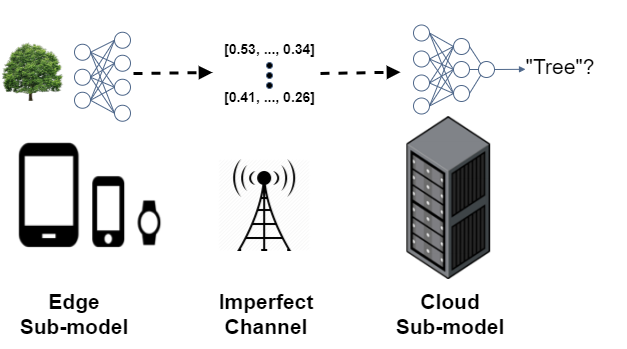
\includegraphics[scale=0.5]{Figures/image--000.png}
	\caption{Blueprint for Collaborative Intelligence.\cite{neurosurgeon}}
	\label{fig:ci}
\end{figure}

\begin{figure}[H]
	\centering
	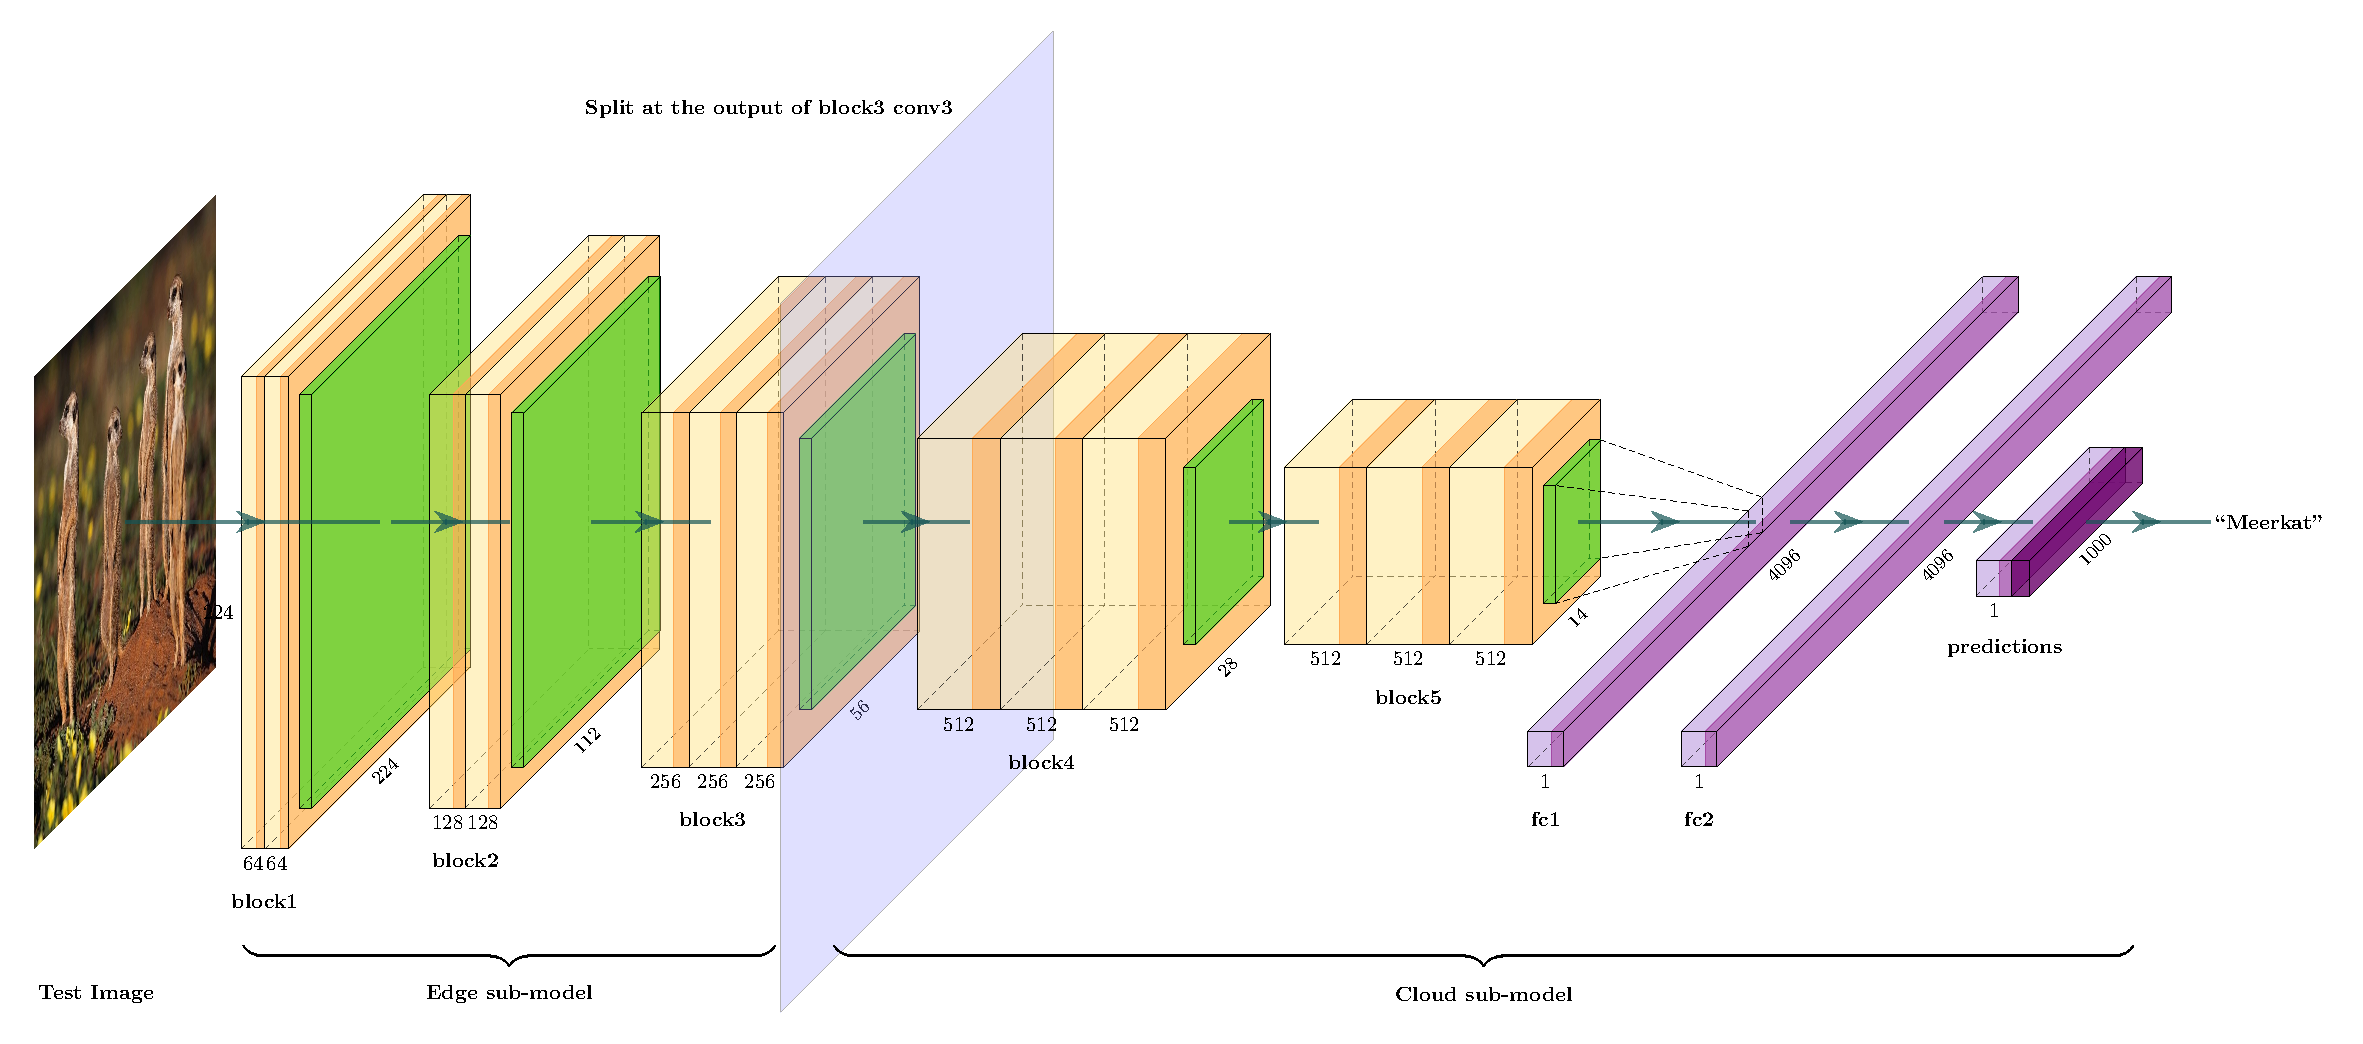
\includegraphics[scale = 0.4]{Figures/vgg16CI.pdf}
	\caption{Splitting a deep model into two sub-models: the mobile or device sub-model and the remote or cloud sub-model.}
	\label{fig:splitting}
\end{figure}

\section{Project overview}

\newpage
\chapter{Background and Literature Survey}
\chapter{Background and Literature Survey} \label{chapter:background}

\section{Collaborative Intelligence} \label{sec:background:ci}


The pioneer papers are \cite{jointdnn} and \cite{neurosurgeon}.


\section{Deep Feature Transmission Simulator} \label{sec:background:dfts}

\gls{dfts} short write up \cite{unnibhavi2018dfts}.

\section{Tensor completion methods} \label{sec:background:tc}

Tensor completion methods for collaborative intelligence \cite{9017944}. Original paper for \gls{silrtc} and \gls{halrtc} \cite{liu2012tensor}.


\hl{say that the algorithms are in appendix}

\section{Summary} \label{sec:background:summary}

\newpage
\chapter{Methods}
\chapter{Methods} \label{chapter:methods}

\section{Introduction} \label{sec:methods:intro}

\section{Summary} \label{sec:methods:summary} 

\newpage
\chapter{Experiments and Results}
\chapter{Experiments and Results} \label{chapter:expts}

\section{Introduction} \label{sec:expts:intro}

\section{Summary} \label{sec:expts:summary}

\newpage
\chapter{Analysis}
\chapter{Analysis} \label{chapter:analysis}

\newpage
\section{Conclusions}
\section{Conclusions and Future Work} \label{chapter:conclusions}

\newpage
\addcontentsline{toc}{section}{References}
\bibliographystyle{ieeetr}
\bibliography{refs}

\end{document}
